\section{Barbershop}
Il problema del Barbiere formato da 2 tipi di processi, un processo barbiere che effettua tagli di barba/capelli a dei processi clienti, e un insieme di processi clienti che vogliono effettuare un taglio. Il negozio del barbiere prevede l'esistenza di una sala d'attesa con n sedie, e la stanza del barbiere con una sedia dove viene effettuato il taglio. Se non ci sono clienti che aspettano di essere serviti, il barbiere dorme. Se arriva un cliente nel negozio vi sono tre casi possibili; tutte le sedie sono occupate da altri clienti, e quindi il cliente se ne va dal negozio, oppure il barbiere è occupato e c'è almeno una sedia libera nella sala d'attesa, il cliente può sedersi ed aspettare che il barbiere si liberi ed effettui il taglio, infine se il barbiere sta dormendo, il barbiere si sveglierà e effettuerà il taglio al cliente.

É importante rispettare i seguenti vincoli:

\begin{itemize}
	\item I processi cliente dovrebbero ricevere il taglio;
	\item Se un cliente arriva quando il negozio è pieno, se ne va;
	\item Il barbiere dovrebbe effettuare i tagli;
	\item Il barbiere serve i clienti uno per volta.
	
\end{itemize}

\subsection{Una possibile soluzione}
Il libro Little Book of Semaphores suggerisce la seguente soluzione: 

Sia n = 2, quindi una sedia per la sala d'attesa e una per la barberia. 

Si vuole utilizzare un mutex per proteggere la sezione critica al cui interno vi è un contattore di clienti presenti nel negozio. Quindi il contattore per essere modificato si dovrà garantire la mutua esclusione. Quando un cliente entra nel negozio dovrà entrare nella sezione critica per controllare che il contattore sia uguale a n, se lo è allora esce dal negozio, se invece non lo è incrementa il contattore ed esce dalla sezione critica. Una volta incrementato il cliente segnala attraverso un semaforo Customer la sua presenza al barbiere e si mette in attesa nel semaforo Barber per attendere il servizio del barbiere.

Una volta che il barbiere segnala la presa in carico del cliente sul semaforo Barber, viene effettuato il taglio e il cliente e il barbiere si sincronizzano sui semafori CustomerDone e BarberDone per garantire che il taglio sia stato fatto e che il barbiere possa effettuare un taglio ad un altro cliente in attesa se c'è altrimenti torna a dormire. Il cliente dopo il taglio entra di nuovo nella sezione critica per decrementare il contattore in modo tale da uscire dal negozio.

Il barbiere nello specifico all'inizio rimane in attesa sul semaforo Customer aspettando l'arrivo di un cliente ( simula il fatto che stia dormendo), una volta svegliato, segnala sul semaforo Barber di essere pronto con il taglio e prendere in carico un cliente(il primo che sincronizza con il segnale), effettua il taglio si sincronizza con il cliente che ha ricevuto il servizio. Se ci sono altri clienti in attesa passa direttamente al nuovo lavoro da effettuare senza mettersi a dormire, invece se non c'è nessuno torna a dormire e si ferma sul semaforo Customer.

\pagebreak
Di seguito viene mostrata una possibile soluzione in pseudo-codice.


\begin{figure}[h]
	\centering
	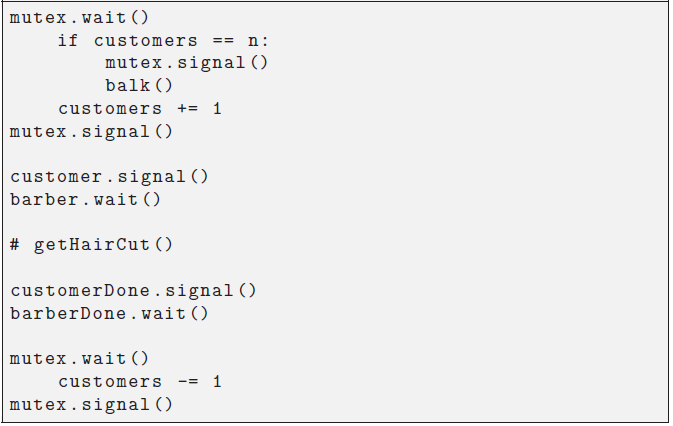
\includegraphics[width=0.6\textwidth]{Figure/2.png}
	\caption{Definizione processo cliente.}
%	\label{fig:baltdx}
\end{figure}

\begin{figure}[h]
	\centering
	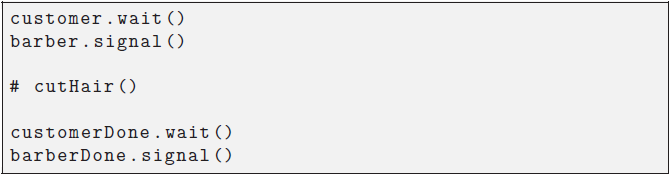
\includegraphics[width=0.6\textwidth]{Figure/3.png}
	\caption{Definizione processo barbiere.}
	%	\label{fig:baltdx}
\end{figure}
\subsection{Modellazione in CCS}

Quindi le entità utilizzate nel programma CCS sono:
\begin{itemize}
	\item Customer$_{i}$: Processo cliente che riceve il taglio;
	\item Count$_{i}$: Mutex con al suo interno il contattore del numero di clienti presenti nel negozio;
	\item Barber: Processo barbiere che effettua il taglio;
	\item Sys: Sistema.
\end{itemize}

Di seguito si mostra un esempio del sistema con n = 2 e tre clienti.

Count1 = enter.incExit.Count2;\\
Count2 = enter.(incExit.CountB + decExit.Count1);\\
CountB = enter.(balk.CountB + decExit.Count2);\\

Customer1 ='enter.('incExit.C1 + 'balk.Customer1);\\
C1 = semCustomer.'semBarber.semCustomerDone.'semBarberDone.'enter.'decExit.Customer1;\\

Customer2 = 'enter.('incExit.C2 + 'balk.Customer2);\\
C2 = semCustomer.'semBarber.semCustomerDone.'semBarberDone.'enter.'decExit.Customer2;\\

Customer3 = 'enter.('incExit.C3 + 'balk.Customer3);\\
C3 = semCustomer.'semBarber.semCustomerDone.'semBarberDone.'enter.'decExit.Customer3;\\

Barber = 'semCustomer.semBarber.'semCustomerDone.cutDone.semBarberDone.Barber;

set L = \{ enter, incExit, decExit, balk, semCustomer, semCustomerDone, semBarber, semBarberDone\};

Sys = (Customer1|Customer2|Customer3|Count1|Barber) \textbackslash L;\\

\subsubsection{Codifica Mutex e contattore clienti}

Per codificare il contattore e il mutex si è deciso di utilizzare un unico processo, o meglio un insieme di processi che codificano il mutex e il contattore, perciò abbiamo: 

\emph{Count1 = enter.incExit.Count2;}

Codifica il contatore che passa da zero a uno gestendo il tutto in mutua esclusione. Per interagire con il contattore i processi clienti devono sincronizzarsi su enter che risulta essere un canale ristretto, ciò permette la mutua esclusione che sarà dimostrata in seguito. Per poter incrementare il contattore e uscire dalla sezione critica i processi cliente utilizzeranno il canale incExit anch'esso ristretto, mentre il processo Count1 andrà nel processo Count2 per mantenere il contatore a uno e per dare la possibilità di decrementare o incrementare un successivo processo cliente.

\emph{Count2 = enter.(incExit.CountB + decExit.Count1);}

Codifica il contatore che passa da uno a due e/o da uno a zero, gestendo il tutto in mutua esclusione. Analogamente a Count1 c'è enter per la sincronizzazione in mutua esclusione. Viene data una scelta in più su come proseguire l'esecuzione. A seconda di cosa richiede il processo cliente può essere data la possibilità di incrementare il contattore e uscire, sempre attraverso il canale incExit, oppure il decremento attraverso decExit(canale ristretto). La scelta dipende dello stato d'esecuzione in cui si trova il processo cliente. Nel caso incrementi, Count2 va in CountB altrimenti torna in Count1.

\emph{CountB = enter.(balk.CountB + decExit.Count2);}

Codifica il contatore che non può essere più incrementato perché uguale a n, e l'azione di decremento. Il funzionamento è uguale a Count2 tranne per il fatto che incExit non esiste ma c'è balk(canale ristretto) usato per simulare l'uscita dal locale del cliente nel caso in cui voglia ricevere un taglio ma non ci sono sedie disponibili.

\subsubsection{Codifica Customer}

La codifica dei clienti avviene nel seguente modo:

\emph{Customer1 ='enter.('incExit.C1 + 'balk.Customer1);}\\
\emph{C1 = semCustomer.'semBarber.semCustomerDone.'semBarberDone.'enter.'decExit.Customer1;}

Il cliente per poter controllare se può entrare si sincronizza sul canale enter rimando in attesa della possibilità di entrare nella sezione critica. Una volta entrato controlla se può incrementare oppure no il contattore, quindi sceglie se eseguire incExit o back, tale scelta dipende da cosa offre il processo count. Nel caso sia CountB, l'unica azione possibile per il cliente è eseguire balk che lo fa uscire dalla sezione critica e non lo fa entrare nel negozio. Nel caso invece sia Count1 o Count2 il cliente esegue incExit cosi che incrementi il contattore e esca dalla sezione critica. Successivamente si sincronizza con il barbiere, che nel caso in cui il barbiere sia libero passa a ricevere il taglio. Finito il taglio si sincronizza subito con il barbiere per poi entrare nella sezione critica in mutua esclusione e decrementare il contattore per simulare la sua uscita dal negozio.

\subsubsection{Codifica Barber}

La codifica del Barbiere avviene nel seguente modo:

\emph{Barber = 'semCustomer.semBarber.'semCustomerDone.cutDone.semBarberDone.Barber;}

Il barbiere rimane in attesa di un nuovo cliente da servire su semCustomer se non ci sono cliente in attesa. Una volta arrivato un cliente si sincronizza con esso ed esegue il taglio, successivamente si sincronizza con il cliente appena servito per garantire che sia avvenuto il taglio per poi tornare all'inizio della sua esecuzione per poter eseguire un nuovo cliente se c'é, altrimenti attende un nuovo cliente.

\subsubsection{Codifica del sistema}

L'intero sistema viene codificato nel seguente modo:

Sys = (Customer1|Customer2|Customer3|Count1|Barber) \textbackslash L;\\
set L = \{ enter, incExit, decExit, balk, semCustomer, semCustomerDone, semBarber, semBarberDone\};

Il sistema viene rappresentato attraverso una composizione parallela dei processi Customer, Barber e Count1. Tutti i canali vengono ristretti per permettere la sincronizzazione dei processi, escluso cutDone usato per mostrare un comportamento all'esterno.

\subsection{Verifica della correttezza attraverso CWB }

Di seguito si verificano se il programma definito rispetta tutte le caratteristiche stabilite dalla definizione del problema, attraverso l'uso della Edinburgh Concurrency Workbench (CWB).

\subsubsection{Weak Bisimulation and Trace Equivalence} 

Spec = cutDone.Spec;

\subsubsection{Assenza di deadlock}

\subsubsection{Mutua esclusione contattore}

\subsubsection{Mutua esclusione nell'esecuzione del taglio}

\subsubsection{Verifica comportamento del cliente che entra quando il negozio pieno}

\subsubsection{Verifica comportamento del barbiere nell'attesa dell'arrivo di un nuovo cliente }

\subsubsection{Verifica comportamento del cliente nell'attesa di essere servito }

\subsubsection{Fairness}



